\documentclass{standalone}
\usepackage{tikz}
\usepackage{pgfplots}
\usetikzlibrary{positioning,3d,decorations.markings,calc}
\pgfplotsset{compat=1.18}

\begin{document}
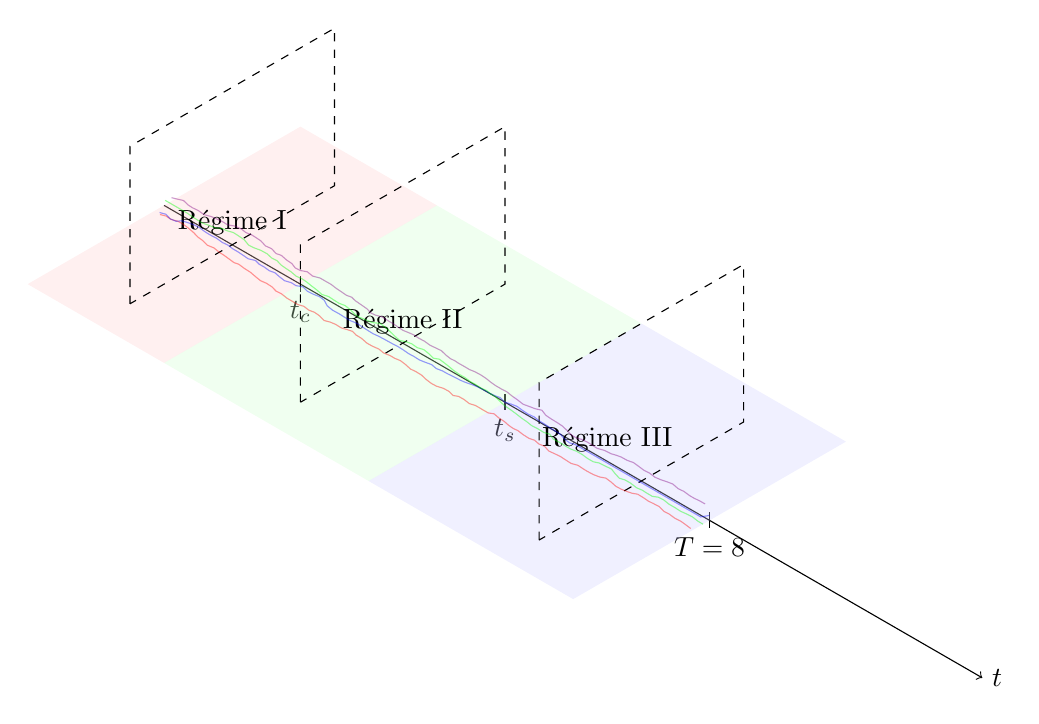
\begin{tikzpicture}[
    x={(0.866cm,-0.5cm)},
    y={(0.866cm,0.5cm)},
    z={(0cm,1cm)}
]
    % Axe temporel
    \draw[->] (0,0,0) -- (12,0,0) node[right] {$t$};
    
    % Points temporels importants
    \draw (8,0,0.1) -- (8,0,-0.1) node[below] {$T=8$};
    \draw (5,0,0.1) -- (5,0,-0.1) node[below] {$t_s$};
    \draw (2,0,0.1) -- (2,0,-0.1) node[below] {$t_c$};
    
    % Zones de régimes colorées
    \fill[blue!20,opacity=0.3] (8,-2,0) -- (8,2,0) -- (5,2,0) -- (5,-2,0) -- cycle; % Régime III
    \fill[green!20,opacity=0.3] (5,-2,0) -- (5,2,0) -- (2,2,0) -- (2,-2,0) -- cycle; % Régime II
    \fill[red!20,opacity=0.3] (2,-2,0) -- (2,2,0) -- (0,2,0) -- (0,-2,0) -- cycle; % Régime I
    
    % Labels des régimes
    \node[above] at (6.5,0,0) {Régime III};
    \node[above] at (3.5,0,0) {Régime II};
    \node[above] at (1,0,0) {Régime I};

    % Encarts pour les coupes (y,z) - maintenant perpendiculaires à l'axe du temps
    \draw[dashed] (1,-1.5,0) -- (1,-1.5,2) -- (1,1.5,2) -- (1,1.5,0) -- cycle; % Encart Régime I
    \draw[dashed] (3.5,-1.5,0) -- (3.5,-1.5,2) -- (3.5,1.5,2) -- (3.5,1.5,0) -- cycle; % Encart Régime II
    \draw[dashed] (7,-1.5,0) -- (7,-1.5,2) -- (7,1.5,2) -- (7,1.5,0) -- cycle; % Encart Régime III

    % Trajectoire 1 (rouge)
    \draw[red,opacity=0.4] plot coordinates {
        (0,-0.06012,-0.08552) (0.08,-0.0528,-0.06828) (0.16,-0.05544,-0.07096) (0.24,-0.0376,-0.06228)
        (0.32,-0.04288,-0.05612) (0.40,-0.04816,-0.0614) (0.48,-0.0454,-0.08304) (0.56,-0.06492,-0.0894)
        (0.64,-0.07636,-0.08584) (0.72,-0.08664,-0.10184) (0.80,-0.07008,-0.1044) (0.88,-0.06932,-0.12052)
        (0.96,-0.07548,-0.11924) (1.04,-0.08848,-0.115) (1.12,-0.09528,-0.11828) (1.20,-0.10208,-0.09732)
        (1.28,-0.10224,-0.10932) (1.36,-0.09292,-0.12312) (1.44,-0.09056,-0.14528) (1.52,-0.1056,-0.14308)
        (1.60,-0.09724,-0.14112) (1.68,-0.09856,-0.14452) (1.76,-0.11528,-0.15268) (1.84,-0.12048,-0.14072)
        (1.92,-0.1166,-0.16068) (2.00,-0.11292,-0.165) (2.08,-0.1206,-0.15808) (2.16,-0.10892,-0.14756)
        (2.24,-0.11844,-0.15104) (2.32,-0.11468,-0.14004) (2.40,-0.12008,-0.14212) (2.48,-0.1326,-0.15564)
        (2.56,-0.12344,-0.14032) (2.64,-0.12424,-0.12896) (2.72,-0.12016,-0.13624) (2.80,-0.11604,-0.11884)
        (2.88,-0.11648,-0.10116) (2.96,-0.14612,-0.09184) (3.04,-0.14512,-0.09524) (3.12,-0.14408,-0.11772)
        (3.20,-0.14656,-0.11368) (3.28,-0.12984,-0.11956) (3.36,-0.139,-0.12524) (3.44,-0.12864,-0.12152)
        (3.52,-0.13464,-0.11568) (3.60,-0.13352,-0.10476) (3.68,-0.14148,-0.10844) (3.76,-0.14592,-0.125)
        (3.84,-0.14256,-0.12204) (3.92,-0.14252,-0.12472) (4.00,-0.15852,-0.12948) (4.08,-0.1624,-0.13856)
        (4.16,-0.1642,-0.13396) (4.24,-0.14288,-0.132) (4.32,-0.13996,-0.13284) (4.40,-0.16168,-0.13312)
        (4.48,-0.161,-0.10528) (4.56,-0.16316,-0.10184) (4.64,-0.16356,-0.11508) (4.72,-0.15064,-0.10656)
        (4.80,-0.14168,-0.11688) (4.88,-0.1258,-0.13272) (4.96,-0.11916,-0.10792) (5.04,-0.13036,-0.11436)
        (5.12,-0.12924,-0.12004) (5.20,-0.1468,-0.11928) (5.28,-0.1588,-0.11392) (5.36,-0.1692,-0.09636)
        (5.44,-0.17808,-0.1) (5.52,-0.16888,-0.11396) (5.60,-0.16628,-0.09916) (5.68,-0.18448,-0.09708)
        (5.76,-0.18156,-0.0882) (5.84,-0.19552,-0.10316) (5.92,-0.18964,-0.0998) (6.00,-0.1868,-0.09588)
        (6.08,-0.19448,-0.09324) (6.16,-0.19116,-0.10132) (6.24,-0.17008,-0.09596) (6.32,-0.18356,-0.08856)
        (6.40,-0.19456,-0.07964) (6.48,-0.18148,-0.08892) (6.56,-0.17056,-0.08424) (6.64,-0.16128,-0.0628)
        (6.72,-0.16404,-0.07132) (6.80,-0.17412,-0.08056) (6.88,-0.17496,-0.07668) (6.96,-0.17184,-0.06732)
        (7.04,-0.17168,-0.05088) (7.12,-0.17468,-0.02012) (7.20,-0.1676,-0.0298) (7.28,-0.17972,-0.02436)
        (7.36,-0.18224,-0.01628) (7.44,-0.17692,-0.01708) (7.52,-0.18648,-0.03424) (7.60,-0.19152,-0.02456)
        (7.68,-0.18912,-0.03864) (7.76,-0.18716,-0.03428) (7.84,-0.19716,-0.03256) (7.92,-0.19648,-0.04548)
    };

    % Trajectoire 2 (bleu)
    \draw[blue,opacity=0.4] plot coordinates {
        (0,-0.06568,-0.05756) (0.08,-0.05344,-0.04564) (0.16,-0.06904,-0.05624) (0.24,-0.0632,-0.05044)
        (0.32,-0.05736,-0.00684) (0.40,-0.05092,0.006) (0.48,-0.04012,0.01336) (0.56,-0.04368,0.02196)
        (0.64,-0.05244,0.01928) (0.72,-0.05792,0.0202) (0.80,-0.03172,-0.00092) (0.88,-0.02396,-0.01916)
        (0.96,-0.02932,-0.00684) (1.04,-0.02856,-0.01904) (1.12,-0.03668,-0.01136) (1.20,-0.04492,-0.00892)
        (1.28,-0.0444,-0.01628) (1.36,-0.02016,-0.00912) (1.44,-0.04308,-0.007) (1.52,-0.05056,0.00264)
        (1.60,-0.05952,0.00136) (1.68,-0.0538,0.01112) (1.76,-0.0674,0.00736) (1.84,-0.07276,-0.00004)
        (1.92,-0.0528,0.00456) (2.00,-0.06704,0.01492) (2.08,-0.04304,0.0266) (2.16,-0.06024,0.02112)
        (2.24,-0.04592,0.01312) (2.32,-0.04088,0.02188) (2.40,-0.05136,0.0212) (2.48,-0.08804,0.00964)
        (2.56,-0.09088,-0.00448) (2.64,-0.07244,-0.02068) (2.72,-0.0774,-0.0192) (2.80,-0.06112,-0.03544)
        (2.88,-0.04796,-0.03532) (2.96,-0.05904,-0.03008) (3.04,-0.0568,-0.03688) (3.12,-0.056,-0.04124)
        (3.20,-0.05472,-0.03376) (3.28,-0.03676,-0.04776) (3.36,-0.01264,-0.06984) (3.44,-0.01436,-0.0632)
        (3.52,-0.0112,-0.07024) (3.60,-0.01352,-0.0758) (3.68,-0.0202,-0.0662) (3.76,-0.01616,-0.07404)
        (3.84,-0.006,-0.07056) (3.92,0.0032,-0.06344) (4.00,-0.00616,-0.06976) (4.08,0.00228,-0.06288)
        (4.16,0.00204,-0.06152) (4.24,0.01652,-0.06824) (4.32,0.02268,-0.07052) (4.40,0.02024,-0.05808)
        (4.48,0.02956,-0.04888) (4.56,0.04432,-0.04864) (4.64,0.05204,-0.05216) (4.72,0.05572,-0.05364)
        (4.80,0.0568,-0.04688) (4.88,0.04756,-0.02324) (4.96,0.03616,-0.03696) (5.04,0.04928,-0.028)
        (5.12,0.05636,-0.02088) (5.20,0.0562,-0.03104) (5.28,0.05708,-0.03872) (5.36,0.06808,-0.04036)
        (5.44,0.05876,-0.044) (5.52,0.06344,-0.0504) (5.60,0.05412,-0.04764) (5.68,0.05688,-0.05336)
        (5.76,0.05156,-0.05072) (5.84,0.0352,-0.06668) (5.92,0.02704,-0.06908) (6.00,0.03056,-0.0524)
        (6.08,0.03056,-0.0524) (6.16,0.03056,-0.0524) (6.24,0.03056,-0.0524) (6.32,0.03056,-0.0524)
        (6.40,0.03056,-0.0524) (6.48,0.03056,-0.0524) (6.56,0.03056,-0.0524) (6.64,0.03056,-0.0524)
        (6.72,0.03056,-0.0524) (6.80,0.03056,-0.0524) (6.88,0.03056,-0.0524) (6.96,0.03056,-0.0524)
        (7.04,0.03056,-0.0524) (7.12,0.03056,-0.0524) (7.20,0.03056,-0.0524) (7.28,0.03056,-0.0524)
        (7.36,0.03056,-0.0524) (7.44,0.03056,-0.0524) (7.52,0.03056,-0.0524) (7.60,0.03056,-0.0524)
        (7.68,0.03056,-0.0524) (7.76,0.03056,-0.0524) (7.84,0.03056,-0.0524) (7.92,0.07536,-0.01472)
    };

    % Trajectoire 3 (vert)
    \draw[green,opacity=0.4] plot coordinates {
        (0,0.01624,0.05604) (0.08,0.01624,0.05604) (0.16,0.01624,0.05604) (0.24,0.01624,0.05604)
        (0.32,0.01624,0.05604) (0.40,0.00852,0.05508) (0.48,-0.00884,0.06956) (0.56,-0.00508,0.06108)
        (0.64,0.01248,0.0624) (0.72,0.0258,0.06316) (0.80,0.04912,0.083) (0.88,0.04632,0.094)
        (0.96,0.0536,0.10948) (1.04,0.04272,0.11724) (1.12,0.05468,0.09736) (1.20,0.04128,0.07428)
        (1.28,0.03824,0.0824) (1.36,0.05524,0.08324) (1.44,0.07368,0.0676) (1.52,0.0544,0.067)
        (1.60,0.05872,0.06664) (1.68,0.03536,0.0656) (1.76,0.0206,0.0732) (1.84,0.02472,0.06256)
        (1.92,0.01892,0.05056) (2.00,0.0182,0.06136) (2.08,0.00708,0.06708) (2.16,0.00108,0.05812)
        (2.24,-0.00016,0.0464) (2.32,-0.0064,0.03284) (2.40,0.0158,0.03324) (2.48,0.00788,0.03568)
        (2.56,0.00664,0.03316) (2.64,0.01356,0.04172) (2.72,0.00756,0.03524) (2.80,0.00448,0.00916)
        (2.88,-0.01268,0.02464) (2.96,0.00592,0.02184) (3.04,0.01244,0.02536) (3.12,0.04728,0.038)
        (3.20,0.04584,0.0272) (3.28,0.02768,0.02952) (3.36,0.01912,0.0134) (3.44,0.0118,0.00116)
        (3.52,0.03088,0.01116) (3.60,0.0308,0.02788) (3.68,0.03168,0.01816) (3.76,0.04888,0.02424)
        (3.84,0.03716,0.02208) (3.92,0.02724,0.00644) (4.00,0.03772,0.02804) (4.08,0.02192,0.03444)
        (4.16,0.01456,0.02892) (4.24,0.00784,0.01912) (4.32,0.0084,0.00972) (4.40,0.01144,0.00916)
        (4.48,0.00876,-0.00112) (4.56,0.00224,0.00744) (4.64,0.00788,-0.0036) (4.72,0.009,0.00488)
        (4.80,-0.00988,0.01104) (4.88,-0.01736,0.01748) (4.96,-0.026,-0.00292) (5.04,-0.0444,-0.0024)
        (5.12,-0.04148,-0.0126) (5.20,-0.03424,-0.0314) (5.28,-0.035,-0.04512) (5.36,-0.04236,-0.0446)
        (5.44,-0.05212,-0.04892) (5.52,-0.04072,-0.05544) (5.60,-0.03128,-0.06824) (5.68,-0.02528,-0.05192)
        (5.76,-0.05324,-0.06096) (5.84,-0.04672,-0.06324) (5.92,-0.04252,-0.07008) (6.00,-0.04152,-0.07184)
        (6.08,-0.02832,-0.06896) (6.16,-0.02448,-0.0736) (6.24,-0.03,-0.07852) (6.32,-0.02556,-0.08328)
        (6.40,-0.02228,-0.0598) (6.48,-0.0124,-0.06348) (6.56,0.00116,-0.06812) (6.64,-0.02188,-0.07952)
        (6.72,-0.04304,-0.08348) (6.80,-0.04284,-0.06452) (6.88,-0.03916,-0.067) (6.96,-0.02976,-0.092)
        (7.04,-0.02708,-0.08328) (7.12,-0.04384,-0.07036) (7.20,-0.04,-0.07504) (7.28,-0.03284,-0.04936)
        (7.36,-0.03076,-0.04656) (7.44,-0.03596,-0.05616) (7.52,-0.02656,-0.06584) (7.60,-0.02576,-0.07124)
        (7.68,-0.02036,-0.06748) (7.76,-0.0086,-0.07324) (7.84,-0.01168,-0.08432) (7.92,-0.01668,-0.08004)
    };

    % Trajectoire 4 (violet)
    \draw[violet,opacity=0.4] plot coordinates {
        (0,0.11028,0.04312) (0.08,0.12012,0.05844) (0.16,0.1248,0.07968) (0.24,0.11604,0.0656)
        (0.32,0.09592,0.08252) (0.40,0.10332,0.08188) (0.48,0.10648,0.06916) (0.56,0.13416,0.07064)
        (0.64,0.1354,0.07884) (0.72,0.14084,0.08136) (0.80,0.13188,0.08672) (0.88,0.1532,0.10192)
        (0.96,0.1712,0.09616) (1.04,0.16,0.09472) (1.12,0.16064,0.10712) (1.20,0.14148,0.1244)
        (1.28,0.13972,0.11956) (1.36,0.12828,0.10084) (1.44,0.13756,0.10168) (1.52,0.12296,0.08704)
        (1.60,0.1192,0.10592) (1.68,0.11624,0.08892) (1.76,0.11348,0.08584) (1.84,0.08296,0.0852)
        (1.92,0.08032,0.09308) (2.00,0.10124,0.10584) (2.08,0.0982,0.09332) (2.16,0.12732,0.094)
        (2.24,0.12748,0.09372) (2.32,0.12972,0.09208) (2.40,0.12324,0.08588) (2.48,0.12288,0.07972)
        (2.56,0.1148,0.08096) (2.64,0.11192,0.09796) (2.72,0.08192,0.11032) (2.80,0.09604,0.08684)
        (2.88,0.09216,0.08264) (2.96,0.07624,0.07384) (3.04,0.06364,0.09368) (3.12,0.07424,0.10804)
        (3.20,0.0824,0.09528) (3.28,0.07648,0.10084) (3.36,0.06264,0.10888) (3.44,0.05992,0.10464)
        (3.52,0.06796,0.10968) (3.60,0.06388,0.1228) (3.68,0.05164,0.12976) (3.76,0.05836,0.12624)
        (3.84,0.06204,0.11212) (3.92,0.07252,0.11) (4.00,0.0666,0.12188) (4.08,0.05864,0.10596)
        (4.16,0.041,0.1128) (4.24,0.02652,0.13264) (4.32,0.00296,0.15184) (4.40,0.00536,0.15076)
        (4.48,-0.0008,0.15528) (4.56,-0.00124,0.16776) (4.64,0.00008,0.16944) (4.72,-0.00404,0.1688)
        (4.80,-0.00056,0.14944) (4.88,-0.0158,0.15788) (4.96,-0.01388,0.1558) (5.04,-0.01368,0.15972)
        (5.12,-0.0198,0.15092) (5.20,-0.01756,0.13984) (5.28,-0.01296,0.1206) (5.36,-0.00132,0.12592)
        (5.44,0.0016,0.13704) (5.52,0.02044,0.14852) (5.60,-0.0004,0.13404) (5.68,-0.00748,0.13436)
        (5.76,-0.0016,0.12612) (5.84,0.00052,0.1176) (5.92,-0.0064,0.10168) (6.00,-0.01684,0.08636)
        (6.08,-0.02788,0.09828) (6.16,-0.03864,0.12808) (6.24,-0.03304,0.13016) (6.32,-0.04276,0.13808)
        (6.40,-0.04928,0.13948) (6.48,-0.02032,0.1384) (6.56,-0.00732,0.13044) (6.64,-0.00772,0.15048)
        (6.72,-0.0148,0.17096) (6.80,-0.0068,0.1646) (6.88,0.00036,0.1756) (6.96,0.0074,0.15784)
        (7.04,-0.00084,0.15504) (7.12,-0.00168,0.16208) (7.20,0.00032,0.14696) (7.28,0.00464,0.15388)
        (7.36,0.01096,0.16608) (7.44,0.0204,0.17128) (7.52,0.0196,0.15248) (7.60,0.02448,0.15484)
        (7.68,0.02756,0.1404) (7.76,0.01532,0.15232) (7.84,0.01488,0.16004) (7.92,0.0152,0.16036)
    };

\end{tikzpicture}
\end{document}
